
\section{Imaging of Brain Activation}

The metabolic changes associated with the hemodynamic response can be imaged through the use of fMRI \cite{Glover2011}. The following section will introduce the concept of fMRI and its use to study brain activation. Before reading this section, it is assumed that the reader is familiar with the basic physics of nuclear magnetic resonance imaging and image reconstruction. If not, an overview can be found in the appendices \ref{sec:physics} and \ref{sec:IMrec}. \\
The fundamental factor that allows fMRI to image brain activity indirectly relies on the measure of the magnetic properties of blood. MRI is dependent on the magnetic susceptibility of the tissues. Local changes in susceptibility results in changes in the MR signal. \cite{Syed2015} Changes in susceptibility arise with the hemodynamic response as oxygenated hemoglobin $(HbO_2)$ is diamagnetic, and de-oxygenated hemoglobin $(Hb)$ is highly paramagnetic as it has four unpaired electrons. The difference in magnetic properties of blood results in what is known as the Blood Level Oxygen Dependent (BOLD) contrast. Thus, as presented in the prior section, the increase in neural activity increases the blood flow to an extend greater than the metabolic utilization of oxygen, which results in a high $(HbO_2)$ to $(Hb)$ ratio. This makes up the difference in BOLD contrast. \cite{Glover2011,Poldrack2011,Khanna2015} \Figref{fig:back:bold} illustrates how the BOLD contrast is dependent on the amount of oxygenated hemoglobin. 

\begin{figure}[H]                 
	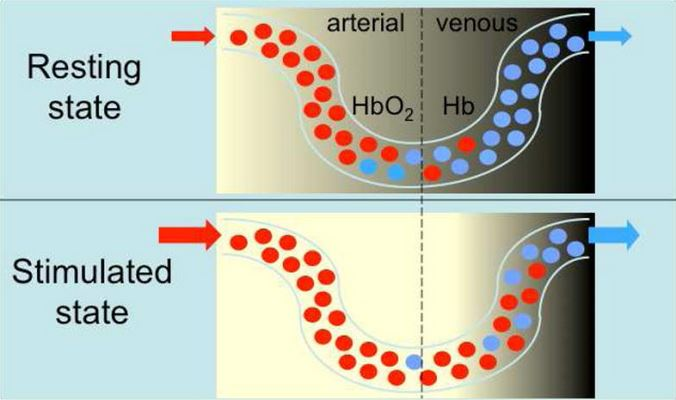
\includegraphics[width=.47\textwidth]{figures/aBackground/bold_response}  
	\caption{Illustration of the concentration difference in oxygenated $(HbO_2)$ and de-oxygenated hemoglobin $(Hb)$ during resting state and stimulated state. The diamagnetic properties of oxygenated blood changes the local magnetic substitutability facilitating a greater contrast change. Illustration taken from \cite{Glover2011}.}
	\label{fig:back:bold} 
\end{figure}

The changes in the BOLD contrast can be recorded by using a $T_{2}^*$ sequence, which is sensitive in detecting changes in the magnetic field. The areas highly filled with oxygenated blood will result in a higher signal in the $T_{2}^*$-weighted sequence making these appear brighter in the reconstructed image. To capture the changes in blood flow over time the acquisitions have to be relatively fast. To achieve fast sequences, the result is a sacrifice of spatial resolution for temporal resolution. \cite{Khanna2015,Lee2002} \\ 
Other methods such as the arterial spin labeled (ASL) method accentuates the functionality of the brain, but BOLD is favored, because it offers a higher contrast-to-noise ratio. \cite{Lee2002} \\ As fMRI can be used as an indirect measure of the neurological response it can capture an individual’s brain activity associated with noxious pain stimuli. Thus, fMRI can be used as a tool to facilitate the understanding of differences between individual’s pain perception.  
%As fMRI can capture the neurological response to pain through the hemodynamic response a measure to study the individual's response to pain is thereby derived. To know more of how the individual's perception of pain is measured in general and by fMRI, including the current difficulties, is of great significance.    
